Presentar una serie de ejemplos y ejercicios clásicos, con sus descripciones
caracaterísticas, condiciones iniciales o de frontera.  Una selección 
de teorías, partiendo por ejemplo de las leyes de conservación y de las 
leyes empíricas, Ley de Fourier, Ley de Darcy, Leyes de Maxwell, Leyes 
en el tránsito, flujos en suelos y plantas, circuitos.
Ecuación de Poisson, Ecuación de Onda, etc.

Es importante la explicación de la condiciones de frontera tipo Dirichlet y Neuman.
Posiblemente, en los libros de Heildeberg. También revisar el libro del profesor 
Hernán Estrada.

\section{La derivada}
El modelamiento matemático es una técnica que utilizan principalmente los matemáticos e ingenieros 
para comprender, simular y predecir el comportamiento de sistemas físicos.  Newton fue uno de 
los precursores, buscaba predecir el comportamiento de los cuerpos que se movían, por ejemplo
tratar de explicar la rotación de los planetas alrededor del sol, o un coche que se moviera en una 
dirección particular.  Para tratar de comprender lo que ocurría, inventó algunos conceptos que son 
muy utilizados hoy en día, por ejemplo el concepto de fuerza, y a diferencia de lo que se había planteado
anteriormente, Newton estableció que todo cuerpo tiende a mantener su estado, excepto que haya una
fuerza externa que cambié su estado inicial.  

Estableció entonces tres leyes que rigen los movimientos de los cuerpos, a saber:

\section{Leyes de conservación}
En primer lugar nos vamos a referir a un \textit{sistema cerrado}, que corresponde a una región 
del espacio que tiene fronteras en el cual siempre se conserva alguna cantidad particular, a la cual
le podemos dar una representación numérica.  Para empezar vamos a determinar la ecuación 
de conservación unidimensional de la masa de un gas en un cilindro. El gas fluye en el tubo en la 
dirección positiva de las $x$, tanto la densidad como la velocidad del gas se suponen constantes cuando
cruzan la sección transversal del cilindro como se aprecia en la figura \ref{fig:cilindro01}. La densidad
se define de tal forma que la masa total $u(x,t)$ del gas en algun intervalo dado $\left[a,b\right]$ 
por ejemplo, está dada por la integral de la densidad como en la ecuación \eqref{eq:masatotal01}:
\begin{equation}\label{eq:masatotal01}
u(x,t)=\int_{a}^{b} \rho(x,t)dx
\end{equation}

\begin{figure}\label{fig:cilindro01}
    \centering
    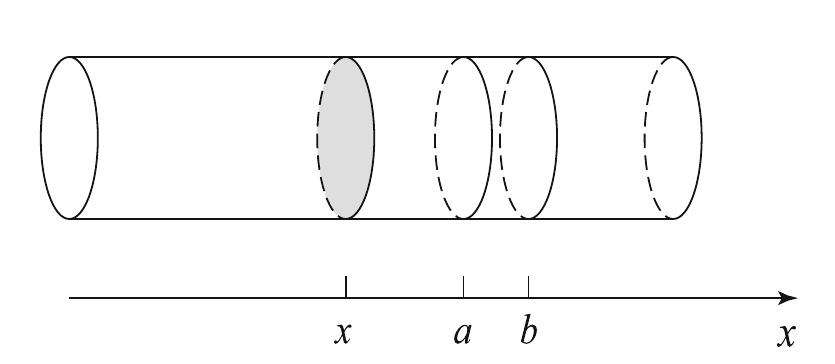
\includegraphics[scale=0.5]{images/cilindro01}
    \caption{Cilindro en el que fluye una masa de gas, en x hay una sección transversal}
\end{figure}

Si suponemos que las paredes del cilindro son impermeables, y la masa del gas ni se crea ni se destruye
al interior del cilindro, entonces la masa en ésta sección sólo puede cambiar debido al flujo del gas
del punto $a$ al punto $b$.

Ahora, supongamos que $v(x,t)$ es la velocidad del gas en el punto $x$ al tiempo $t$.  Entonces la 
velocidad del flujo o el flujo másico $\phi$ que pasa por éste punto estará dado por la ecuación 
\eqref{eq:flujo-masico}:
\begin{equation}\label{eq:flujo-masico}
    \phi(x,t) = \rho(x,t)v(x,t)
\end{equation}
Que al establecer las unidades resulta en la expresión \eqref{eq:unidades01}:
\begin{equation}\label{eq:unidades01}
    \left[\phi\right]=\frac{kg}{s} = \left[\rho\right]\left[v\right]= \frac{kg}{\cancel{cm}}\frac{\cancel{cm}}{s}
\end{equation}

Así el flujo másico tendrá unidades de kilogramos ''$kg$'' por segundo ''$s$'', es decir una medida de la 
cantidad de masa que pasa por cada segundo en un $x$ particular.

Debido a que el flujo másico tiene unidades de kilogramos por segundo, entonces podemos derivar la 
ecuación \eqref{eq:masatotal01} de donde obtenemos la razón de cambio de la masa en el intervalo
$[a,b]$ por la expresión \eqref{eq:cambio_masa}:
\begin{equation}\label{eq:cambio_masa}
    \frac{d u(x,t)}{dt} = \frac{d}{dt}\int_a^b\rho(x,t)dx=\overbrace{\rho(a,t)v(a,t)}^{masa\ que\ entra}
    -\underbrace{\rho(b,t)v(b,t)}_{masa\ que\ sale}
\end{equation}
Que se puede interpretar como, el cambio en la masa en un instante de tiempo, es igual a la cantidad 
de masa que entra en el intervalo, menos la cantidad de masa que sale. La ecuación \eqref{eq:cambio_masa}
es una forma \textbf{integral} de la ley de conservación.
\section{Casos especiales de las leyes de conservación}

\section{Ejemplos de modelos matemáticos}


\section{Aplicaciones}
\subsection{Ecuación de Poisson}
\subsection{Otras aplicaciones}